\documentclass[article]{BJTU-thesis}
\usepackage{url}
\usepackage{booktabs}
\setcounter{tocdepth}{4}
\setcounter{secnumdepth}{4}
\hypersetup{hidelinks}
\renewcommand\thesection{\arabic {section}}
\renewcommand\thefigure{\arabic {figure}}
%%%%%%%%%%%%%%%填写封面信息%%%%%%%%%%%%%%%%%%%%
\authora{汤新宇  17301137}
\authorb{陈嘉琪  17301060}
\authorc{刘歆怡  17301129}
\authord{唐{\color{white}哈}麒  17301138}
\authorf{张钰铎  17301145}
\comment{同{\color{white}哈}等{\color{white}哈}贡{\color{white}哈}献}
%\studentNumber{16121248}
\advisor{冀振燕}
%\advisorTitle{教授}
%\degreeType{学术型}
%\major{机械制造}
%\researchArea{切削力分析}
\title{面向数据的软件体系结构}
\bibliographystyle{unsrt} % BibTex
%\englishtitle{The Path Planning of Blade Machining Tool Based on Cutting Force Analysis.}
%%%%%%%%%%%%%%%%%%%%%%%%%%%%%%%%%%%%%%%%%%%%%%
%\setmainfont{Times New Roman}
\bibliographystyle{unsrt} % BibTex
\begin{document}
	\makecover
	
	\tableofcontents
	\newpage

	\newpage
	\setcounter{page}{1}
	\section{简介}
	
	软件体系结构,是随应用需求不断演变而产生的,如图\ref{fig:fig0}所示。
	\begin{figure}[!htbp]
		\centering
		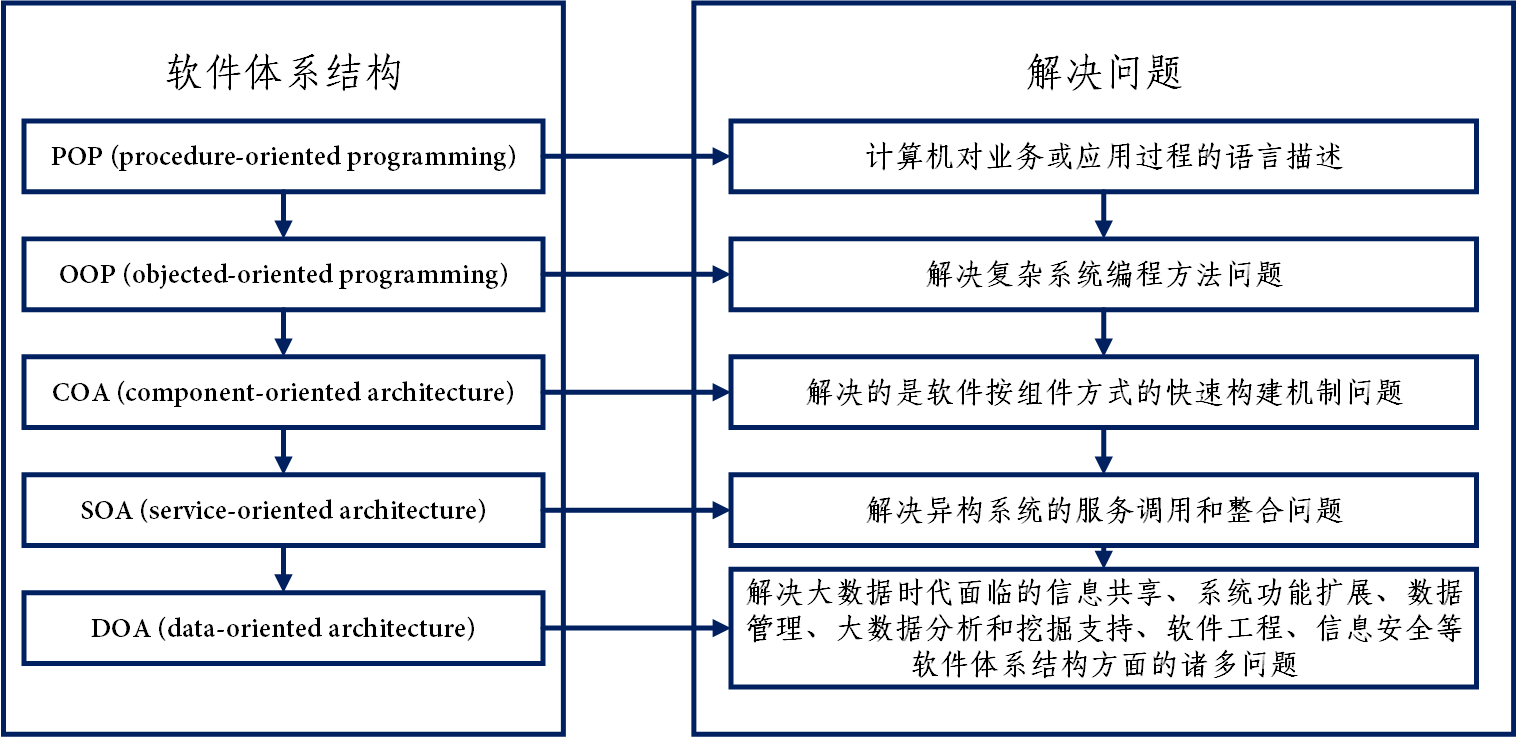
\includegraphics[width=1\textwidth]{0.png}
		\caption{软件体系结构}
		\label{fig:fig0}
	\end{figure}

	受软件体系结构的限制,信息技术领域长期存在的问题在大数据时代愈发突出:系统间的信息难以共
	享;已建系统功能扩展困难;海量、异构、多源、动态、实时变化和爆发式增长的大数据难管理,难分析,难挖掘;面向业务的软件工程开发过程复杂,维护困难,生命周期短;在互联网开放环境下的信息安全、数据安全问题面临挑战;数据所有者利益得不到保障等。
	
	面向数据的软件体系结构(data-oriented software architecture,
	DOA),采用“面向数据和以数据为核心”的思想,通过数据注册中心(data register center,DRC)、数据权限中心data authority center,DAC)和数据异常中心(data exception control center,DEC)统一定义数据、管理数据和提供数据服务;通过数据应用单元(data application units,DAUs)对各种应用进行管理和服务,建立了一种数据大平台与碎片化应用的数据生态系统,为构建大数据时代从数据保护到授权应用整套机制的软件体系结构,进行了有益的探索。
	
	本文将从软件体系结构的发展、面向数据的软件体系结构及其研究进展和面临的问题几个方面进行介绍。
	
	\section{软件体系结构发展历程、现状、发展方向}
	\subsection{软件体系结构发展历史}
	软件系统的规模和复杂度在不断增大的同时,众多软件开发过程和方法相继出现。这一过程中,软件体系结构的研究也由最初模糊的概念发展到一个渐趋成熟的技术。
	
	远在20世纪70年代以前,尤其是在以ALGOL68为代表的高级语言出现以前,软件基本上都是用汇编程序编写的。此阶段系统规模较小,很少明确考虑系统体系结构, 一般不存在系统建模工作。70年代中后期,由于结构化开发方法的出现与广泛应用,软 件开发中出现了概要设计与详细设计,而且主要任务是数据流设计与控制流设计。因此,此时软件结构已作为一个明确的概念出现在系统的开发中。
	
	20世纪80年代初到90年代中期,是面向对象开发方法兴起与成熟阶段。由于对象是数据与基于数据之上操作的封装,因而在面向对象开发方法下,数据流设计与控制流设计则统一为对象建模。同时,面向对象方法还提出了一些其他的结构视图,如在OMT 方法中提出了功能视图、对象视图与动态视图(包括状态图和事件追踪图);而BOOCH方法中则提出了类视图、对象视图、状态迁移图、交互作用图、模块图、进程图;1997年出现的统一建模语言UML则从功能模型(用例视图)、静态模型(包括类图、对象图、构件图、包图)、动态模型(协作图、顺序图、状态图和活动图)、配置模型(配置图)描述应用系统的结构\cite{a}。
	
	90年代以后则是基于构件的软件开发阶段,该阶段以过程为中心,强调软件开发采用构件化技术和体系结构技术,要求开发出的软件具备很强的自适应性、互操作性、可扩展性和可重用性。此阶段中,软件体系结构已经作为一个明确的文档和中间产品存在于软件开发过程中。同时,软件体系结构作为一门学科逐渐得到人们的重视,并成为软件工程领域的研究热点,因而Perry和Wolf认为,``未来的年代将是研究软件体系结构的时代!''。
	
  	进入21世纪10年代,以大数据为特征的新时代已经来临。2011年12月,赵国栋等人发布了《大数据时代的即将到来》的报告,这是中国关于大数据的第一声呐喊;2012年《大数据》和《大数据时代》先后出版;同年12月,鄂维南院士组织召开了第一届数据科学及产业发展大会,中关村大数据产业联盟也成立了;直到2015年5月,贵阳国际大数据博览会成功举办,形成全国性的影响力;2015年9月,国务院发布《促进大数据发展行动纲要》,发展大数据正式成为国家意志,也标志着大数据时代来临。大数据时代下,大数据技术、大数据分析和挖掘,以及数据管理、信息共享、信息安全、软件工程、系统扩展等,已经成为政府、企业界和科技界关注的热点和面临的挑战。李国杰院士在关于大数据应用与研究所面临的问题与挑战中指出,大数据时代,“需要考虑对整个 IT 架构进行革命性的重构”。
  	
  	广义上讲,革命指推动事物发生根本性变革,引起事物从旧制到新制的飞跃。IT架构的革命性重构本文认为应该从硬件和软件两个方面来考虑。云计算已经较好地解决了硬件方面的问题,是目前公认非常高效的处理大数据的方法之一。亚马逊的弹性计算云(elastic compute cloud,EC2)和简单存储服务(simple storage service,S3)是云计算发展的典范;OpenStack 凭借开放先进的架构、高效的社区开发、灵活的部署模式获得了业界的广泛认可,成为当今最有影响力的云计算开源项目;OpenStack 和Hadoop 的融合,既最大限度提高了服务器的资源利用率,又大大降低了大数据储量的准入门槛;NoSQL技术系统解决了类型多样的大数据的管理、处理和分析问题;以MapReduce、Hadoop、Spark等为代表的非关系数据分析技术,快速地借助云计算平台和大数据处理技术把数据转换为商业价值,在互联网搜索和其他大数据分析领域取得了重大进展。
  	
  	云计算为软件方面的革命性重构奠定了重要基础,但在软件的体系结构上,目前还没有很好的解决方案。加拿大实时创新公司(Real-Time Innovation,Inc)的Joshi博士提交了“面向数据的体系结构:松散耦合的实时SOA”白皮书。该作者曾指出:数据是第一位的,对数据的操作是第二位的。但作者只是从系统集成角度开展研究,没有在面向数据方面的后续研究。Mohanty 等人在“Big Imperatives, Enterprise Big Data Warehouse,BI Implementations and Analytics”一书中,讨论了传统的企业数据仓库和大数据仓库储存大数据时面临的挑战,提出通过设计一个混合数据仓库架构来实现数据平台生态系统,体现了部分面向数据的思维。Sawant 等人在“BigData Application Architecture Q\&A”一书中,较深入地探讨了大数据的应用体系结构设计原则和实现方法,明确提出数据作为服务(data as a service, DaaS)对于大数据下的应用架构具有较重要的指导意义。Llopis 等人也在游戏设计领域采用面向数据的设计思想实现产品设计。国内外还有一些相关研究,都不同程度地体现了一些面向数据的思想、大数据的应用架构及相关技术,但均未提出较完整的面向数据的软件理论和方法体系。

	目前有学者在云计算的硬件架构之上,采用“面向数据和以数据为核心”的思想,构建一种适应于大数据时代的面向数据的软件体系结构(data- oriented software architecture,DOA)。DOA 通过数据注册中心(data register center,DRC)、数据权限中心(data authority center,DAC)、数据异常控制中心(data exception control center,DEC)来统一定义数据、管理数据和提供数据服务,通过数据应用单元(data application units,DAUs)对各种应用进行管理和服务,建立一种数据大平台与碎片化应用的可持续发展的数据生态系统,并构建从数据保护到授权应用的整套机制,为有效解决大数据时代所面临的问题和挑战提供基础理论和方法技术支撑。云计算与DOA分别从硬件和软件两个方面,共同构建起大数据时代的 IT基础架构,其特点和优势如表\ref{tab:aStrangeTable}所示。

	\begin{table}[!htbp]
		\centering
		\caption{云计算与DOA的特点和优势}\label{tab:aStrangeTable}
		\begin{tabular}{p{7cm}p{7cm}}
			\toprule
			云计算(虚拟化的硬件体系结构)& DOA(面向数据的软件体系结构)\\
			\midrule
			硬件资源虚拟化& 面向数据和以数据为核心\\
			\midrule
			虚拟化的硬件资源:计算、存储、网络&数据生态系统——数据大平台与碎片化应用:肥沃的数据土壤上生长着茂盛的应用森林\\
			\midrule
			使硬件资源可伸缩、可计量、可管理&数据:天生加密,授权使用\\
			\midrule
			硬件体系结构的革命性重构&软件体系结构的革命性重构\\
			\midrule
			硬件性能方面,能够不断满足业务增长和用户规模扩大&软件功能方面,能够不断满足应用需求变化和数据增长变化\\
			\midrule
			支撑整个信息系统的基础设施&支撑整个数据资源及业务应用的管理\\
			\bottomrule
		\end{tabular}
	
	\end{table}
	
	\subsection{国内外研究现状与进展}
	\subsubsection{国外研究进展}
	1995年出版的IEEE Software体系结构专刊\cite{Garlan1995Introduction}和1996年出版的专著\cite{ShawSoftware} Software Architecture: Perspectives on an Emerging Discipline,可以认为是软件体系结构作为软件工程一个研究方向正式提出的标志。此后软件体系结构领域得到了蓬勃发展。越来越多的研究者关注并参与到软件体系结构的研究中来,与软件体系结构相关的会议、期刊、书籍等逐步增多,越来越多的知名国际会议将软件体系结构列入主要议题,并举行了大 量直接以软件体系结构为主题的研讨会或国际会议(如软件体系结构国际研讨会ISAW, WICSA等)。软件体系结构的研究还得到了工业界的广泛关注与认同,如UML2标准中引入了软件体系结构领域中连接子的概念\cite{Allen1994Formalizing},在实际软件开发过程(如RUP统一软件开发过程\cite{Ivar1999Unified})中也引入软件体系结构的概念和原则。2006年出版的IEEE Software软件体系 结构专刊\cite{Kruchten2006The}总结了十年间软件体系结构研究与实践。Shaw M等在论文中\cite{ShawThe}从技术成熟的六个阶段分析了软件体系结构的进展。下面给出软件体系结构的主要研究内容。
	\newline

	\noindent\textbf{研究内容一:软件体系结构的形式化描述语言}
	
	软件体系结构研究如果仅仅停留在非形式化的框图和文本表示阶段,已经难以适应进一步发展的需要。为支持基于体系结构的开发,需要有形式化建模符号,体系结构描述、测试、评估的自动化工具。从软件体系结构研究的现状来看,在这一领域近来已经有不少进展,其中比较有代表性的是美国卡耐基梅隆大学提出的Wright系统。Wright 是一种结构描述语言,该语言基于一种形式化的、抽象的系统模型,为描述和分析软件体系结构和结构化方法提供了一种实用的工具。目前主要的ADL包括Unicon,Rapide, Darwin, Wright, C2 SADL, Acme, axel\cite{DashofyA},XYZ/ADL, ABC/ADL\cite{Mei2002ABC}等。Medvidovic提出了一套ADL的分类和比较框架,对2000年之前的ADL研究作了较为详尽的总结和评估\cite{Medvidovic2000A}。随着软件体系结构研究的不断深入,研究人员还挖掘出了ADL需要进一步 深入考虑的问题,比如支持动态、分布、移动系统的建模,针对不同应用领域的建模等, 从而提出了一些新型的ADL,比如基于可扩展构件模型Fractal的ADL、从结构和行为 的角度来描述体系结构的n -ADL\cite{Oquendo2004}、基于多Agent系统的Skwyrl-ADL等。软件体系结 构的形式化研究为软件开发和维护提供了强有力的支持。
	
	目前,存在众多的体系结构描述语言,这样势必导致认知和使用上的混乱。同时,每一种ADL都以独立的形式存在,描述语法不同且互不兼容,同时又有许多共同的特征,这使设计人员很难选择一种合适的ADL,若设计特定领域的软件体系结构又需要从头开始描述。学者们认为有必要从元模型层次探讨统一的体系结构描述方式。随着软件系统的不断发展和演化,新的问题也不断涌现,对软件体系结构的形式化描述将一直是研究的热点。
	\newline
	
	\noindent\textbf{研究内容二:软件体系结构的多视图模型表示}
	
	  研究软件体系结构的首要问题是如何表示软件体系结构,即如何对软件体系结构建模。根据建模的侧重点的不同,可以将软件体系结构的模型分为5种:结构模型、框架模型、动态模型、过程模型和功能模型。在这5个模型中,最常用的是结构模型和动态模型。
	  
	\textbf{结构模型:}这是一个最直观、最普遍的建模方法。这种方法以体系结构的构件、连接件和其他概念来刻画结构,并力图通过结构来反映系统的重要语义内容,包括系统的配置、约束、隐含的假设条件、风格、性质。研究结构模型的核心是体系结构描述语言。

	\textbf{框架模型:}框架模型与结构模型类似,但它不太侧重描述结构的细节而更侧重于整体的结构。框架模型主要以一些特殊的问题为目标建立只针对和适应该问题的结构。

	\textbf{动态模型:}动态模型是对结构或框架模型的补充,研究系统的“大颗粒”的行为性 质。动态可能指系统总体结构的配置、建立或拆除通信通道或计算的过程。
	
	\textbf{过程模型:}过程模型研究构造系统的步骤和过程。因而结构是遵循某些过程脚本的结果。
	
	\textbf{功能模型:}该模型认为体系结构是由一组功能构件按层次组成,下层向上层提供服务。它可以看作是一种特殊的框架模型。
	
	这5种模型各有所长,也许将5种模型有机结合起来,形成一个完整的模型来刻画 软件体系结构更合适。通常认为,软件系统存在用例分析模型、静态结构模型、动态行为模型和物理结构模型\cite{Schmuller2004Sams}。如何将这四种模型有效集成,正是软件体系结构模型解决的 问题。例如,Kruchten在1995年提出了一个“4+1”的视角模型(逻辑视角、过程视角、 物理视角、开发视角和场景视角),Homelier的4视图模型(概念视图、模块视图、执行视图、代码视图),CMU-SEI的Views and Beyond模型(模块视图、构件和连接子视图、分配视图)等。此外,工业界也提出了若干多视图描述软件体系结构模型的标准,如IEEE 标准1471-2000(软件密集型系统体系结构描述推荐实践)、开放分布式处理参考模型(RM-ODP)、统一建模语言UML以及IBM公司推出的Zachman框架等。
	\newline
	
	\noindent\textbf{研究内容三:特定领域的软件体系结构}
	
	 经过几十年的软件研究和开发实践。今天人们开发的应用系统很少与过去的软件系统没有联系或相似之处。特别是在某一领域中。不同系统、不同版本之间的软件体系结构是非常相似的。这为基于软件体系结构的重用创造了条件。特定领域软件体系结构 (Domain Specific Software Architecture, DSSA)表示的就是某一特定领域的体系结构,抽象出领域中各应用系统的公共特征与动态行为。作用于领域中各系统,通过大规模重用,可以可靠、高效快速地实例化出一系列软件产品。
	 
	鉴于特定领域的应用具有相似的特征,因而经过严格设计,并将直觉的成分减少到最少程度,可以有效地实现复用,并可借鉴领域中已经成熟的体系结构。特定领域的体系结构是将体系结构理论应用到具体领域的过程。常见的有电信软件的体系结构研究、 CASE体系结构、CAD软件的参考模型、测试环境的体系结构、信息系统的参考体系结构、网络体系结构、机场信息系统的体系结构等。
	\newline
	
	\noindent\textbf{研究内容四:软件产品线体系结构的研究}
	
	 软件体系结构的开发是大型软件系统开发的关键环节。体系结构在软件产品线的开发中具有至关重要的作用。同一个软件体系结构,可以创建具有不同功能的多个系统。在软件产品族之间共享体系结构和一组可重用的构件,可以增加软件重用、降低开发和维护成本。一个产品线代表着一组具有公共的系统需求集的软件系统,它们都是根据基本的用户需求对标准的产品线体系结构进行定制,将可重用构件与系统独有的部分集成而得到的。采用软件生产线式模式进行软件生产,将产生巨型编程企业。但目前生产的软件产品族大部分是处于同一领域的,也就是说软件产品线体系结构可以参照特定领域的软件体系结构。
	\newline
	
	\noindent\textbf{研究内容五:软件体系结构的分析和设计研究}
	
	软件体系结构是对软件系统的高层抽象,是在软件开发过程之初产生的,因此设计优质的体系结构可以减少和避免软件错误的产生和维护阶段的高昂代价。体系结构是系 统集成的蓝本、系统验收的依据,体系结构本身需要分析与测试,以确定这样的体系结构是否满足需求,如非功能分析的体系结构分析方法SAAM (Software Architecture Analysis Method)、基于场景的体系结构分析方法、多质量属性情况下的体系结构质量模型、分析与权衡方法 ATAM (Architecture Tradeoff Analysis Method)。生成一个满足软件需求的体系结构的过程即为体系结构设计,体系结构设计过程的本质在于:将系统 分解成相应的组成成分(如构件、连接件),并将这些成分重新组装成一个系统。体系结构设计有两大类方法:过程驱动方法和检查列表驱动方法。体系结构的分析和设计是软件开发中研究的重点,是体系结构设计者必须要精通的技能,在开发者社区、博客、网站等有相当激烈的讨论。要将体系结构运用到软件开发过程中,分析和设计是第一步,因此,软件体系结构的分析和设计在企业应用开发中得到了相当大的重视。很多实践者通过不同领域应用总结了大量的经验,推动了软件体系结构在开发中的应用研究。
	
	\subsubsection{国内研究进展}
	近年来国内在软件体系结构风格、描述方法、设计方法、基于软件体系结构的构件组装以及软件体系结构测试技术等方面都比较活跃。
	\newline
	
	\noindent\textbf{研究内容一:软件体系结构概念}
	
	 孙昌爱等\cite{b}归纳了软件体系结构技术发展过程及主要研究方向,给出了软件体系结构的定义,提出了软件体系结构研究的两大思路,并从7个方面介绍了软件体系结构研究进展,探讨了软件体系结构研究中的不足之处,给出了软件体系结构领域最有前途的发展趋势。基于软件体结构进十年的研究进展,梅宏等在论文\cite{c}中综述了在软件生命周期的不同阶段软件体系结构的研究与应用,并探讨了软件体系结构领域的发展与研究方向。
	\newline
	
	\noindent\textbf{研究内容二:软件体系结构描述方法}
	
	朱雪阳在论文\cite{d}中提出了双重软件体系结构描述框架 XYZ/ADL,前端用一般的体系结构框图来描述;后端用既可表示系统动态语义又可表示系统静态语义的时序逻辑语言XYZ/E作为一致的语义基础。王晓光等\cite{e}提出了一种基于XML的体系结构描述语言——ABC/ADL。杨敬中等\cite{f}在软件体系结构描述语言XYZ/ADL的基础上,通过增加新的元素和相关复合机制,得到一种面向方面的体系结构描述语言AO-ADL,实现了在软件体系结构中横切功能的模块化。
	\newline
	
	\noindent\textbf{研究内容三:软件体系结构设计}
	
	毛斐巧、李俊娥、汪保杰等人分别对软件体系结构风格应用进行了研究,毛斐巧等人\cite{g}在论文中指出了体系结构风格四个重点研究方向及各自存在的问题。李俊娥等人\cite{h}研究了插件体系结构风格,并给出了插件体系结构风格的描述以及基于插件体系结构风格的开发过程。汪保杰等人\cite{i}在论文中给出正交体系结构风格的概念,并结合系统 案例,给出了正交化简易算法、正交设计过程以及演化方法。
	\newline
	
	\noindent\textbf{研究内容四:软件体系结构测试技术}
	
	近两年也有进一步的研究。目前,一些有代表性的软件测试策略被研究人员提议用于软件体系结构的测试。但是,传统的软件测试技术和方法不能直接用来解决软件体系结构的测试问题,巩绪芳等人在论文\cite{j}中概述了软件体系结构测试策略的研究现状,剖析了影响软件体系结构测试的因素,并讨论了软件体系结构分析与测试的未来研究主题。许慧等人在论文中\cite{k}针对目前体系结构描 述语言对描述软件系统行为方面的不足而难以生成实时测试路径的问题,提出一种基于PI演算的软件体系结构测试方法,该方法包括PI演算与Petri网结合、构造体系结构模型及测试路径生成算法。
	\newline
	
	\noindent\textbf{研究内容五:基于软件体系结构的构件组装技术}
	
	任洪敏等在论文\cite{l}中给出了复合构件和复合接口的组装 推导算法,为系统行为的形式化分析、验证和仿真奠定了基础。向俊莲等在论文\cite{m}中介绍了为ABC方法提供有效支持的工具ABC-Tool,ABC-Tool以软件体系结构为设计蓝图,以构件为基本开发单元,通过可视化的图形建模方式,将可运行或可部署的构件组装为最终可正确运行的系统。
	
	\section{面向数据的软件体系结构}
	\subsection{面向数据的软件体系结构介绍}
	面向数据的体系结构(DOA)建立在云计算的硬件架构之上,采用“面向数据和以数据为核心”的思想,是一种适应于大数据时代的面向数据的软件体系结构(data- oriented software architecture,DOA)。DOA 通过数据注册中心(data register center,DRC)、数据权限中心(data authority center,DAC)、数据异常控制中心(data exception control center,DEC)来统一定义数据、管理数据和提供数据服务,通过数据应用单元(data
	application units,DAUs)对各种应用进行管理和服务,建立一种数据大平台与碎片化应用的可持续发展的数据生态系统,并构建从数据保护到授权应用的整套机制,为有效解决大数据时代所面临的问题和挑战提供基础理论和方法技术支撑。
	
	\begin{figure}[!htbp]
		\centering
		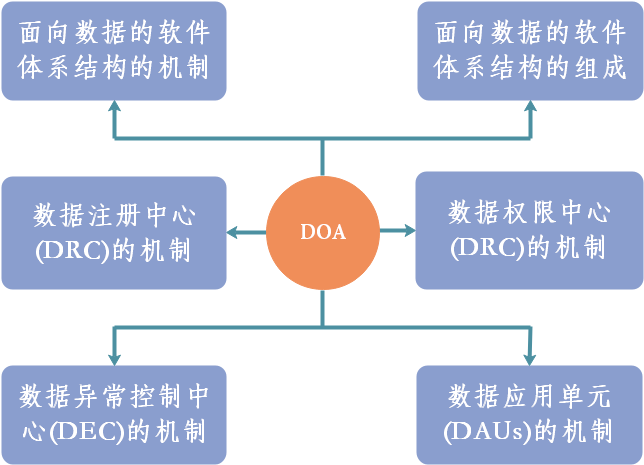
\includegraphics[scale=0.6]{1.png}
		\caption{DOA 的组成部分}
		\label{fig:fig1}
	\end{figure}
	
	\subsubsection{面向数据的软件体系结构的机制}
	\noindent\textbf{(1) 数据的类型}
	
	数据指的是广义数据,是真实世界映射成虚拟世界的内容,可以是数字、文字、设备、服务、APP、人、物等。数据的类型也可以划分成很多种:结构化/非结构化数据,关系型数据库/NoSQL,动态数据/静态数据,变化的数据/历史数据,简单数据/复杂数据,自有数据/共享数据/公开数据,不断变化和不断积累增长的大数据等。
	\newline
	
	\noindent\textbf{(2) 云计算硬件架构基础上的DOA软件架构}
	
	云计算即云服务,可以提供数据的存储服务(IaaS 和DaaS),通过分布式和虚拟化技术,将基础设施与数据融为一体(infrastructure
	plus data,I+D),为终端用户提供弹性、可计量、个性化的数据和计算服务,可以简称“云”。以数据为内容定义云,可以分为存储云、网络云和物理云。DOA就是建立在云计算支撑的数据和各种应用之间的,分别可以对数据和应用进行管理和服务的一种机制、一个平台,形成一个以这种机制和平台的相对不变来应对万变的数据和应用的生态系统。这种关系和机制,也可以实现从实时数据到实时应用的支持。数据、DOA平台和应用所构成的三层架构见图\ref{fig:fig2}。
	
	
	\begin{figure}[!htbp]
		\centering
		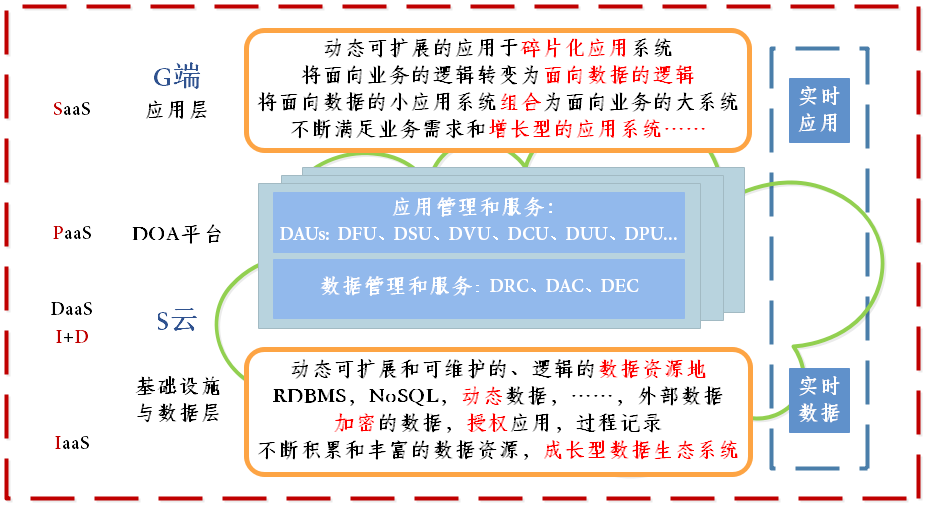
\includegraphics[width=1\textwidth]{2.png}
		\caption{数据、DOA平台和应用所构成的三层架构}
		\label{fig:fig2}
	\end{figure}
	
	\noindent\textbf{(3) DOA对数据的管理和服务模式}
	
	DOA对广义数据进行管理,首先要解决对各种类型数据的统一标识问题。其次,要考虑数据的价值保护,对数据进行属性管理,并对数据进行权限和授权管理。第三,在分布式应用和有数据冗余的情况下,要考虑数据的唯一性和一致性问题。据此提出DRC、DAC 和DEC,互相配合实现对各种类型数据的统一管理,并为应用提供数据服务。
	\newline
	
	\noindent\textbf{(4) DOA 与应用的业务逻辑和数据逻辑关系}
	
	面向数据的软件体系结构,首先应将应用的业务逻辑转换为数据逻辑,即将业务流程按照对数据资源池访问的周期梳理成一个个小的面向数据的流程,最后再将这些面向数据的流程整合成面向业务的流程,完成应用信息系统的开发。区别于传统面向业务的逻辑,面向数据的逻辑带来的好处是:构建了数据资源池,构建面向数据的业务流程会比较便捷,而且业务流程发生变化,不会影响整个数据逻辑和数据流程,只需增加变化的部分或调整一些数据流程去适应新的变化即可。
	
	\subsection{DOA与SOA的比较}
	\subsubsection{面向服务的软件体系结构(SOA)}
	
	\begin{figure}[!htbp]
		\centering
		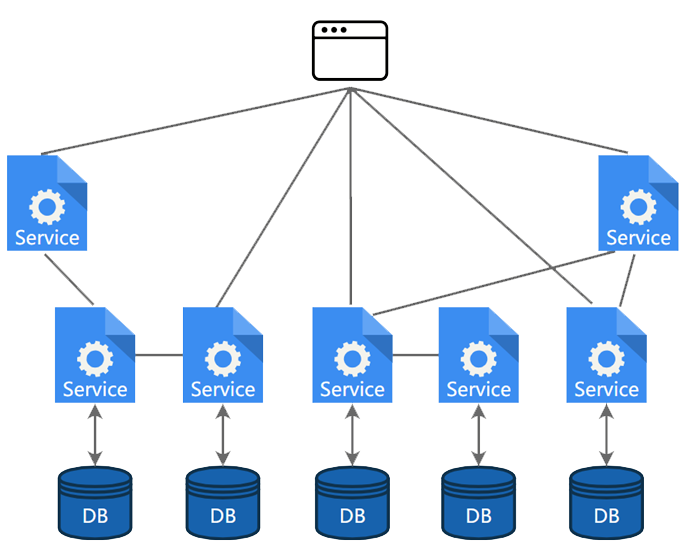
\includegraphics[scale=0.8]{3.png}
		\caption{SOA的拓扑结构}
		\label{fig:fig3}
	\end{figure}
	
	面向服务的体系结构可以根据需要,独立(并行)开发和推进不同的服务。这些服务是松耦合的,这意味着一个全新的服务可以重用其他的服务。
	
	SOA中的每个服务都定义了自己的API,因此可以独立访问每个服务并与之交互。调试或开发单个组件的人员可以分别调用单个组件,重新组合这些单个服务,创建新的工作流。
	
	在SOA中,各个组件通过每个组件定义的API彼此直接通信。为了进行通信,每个组件都是可单独寻址的(即使用IP地址,服务地址或其他内部标识符来回发送请求/消息)。这意味着体系结构中的每个组件都需要了解其依赖关系,并且需要专门与它们集成。
	
	\subsubsection{面向对象的软件体系结构(DOA)}
	
	\begin{figure}[!htbp]
		\centering
		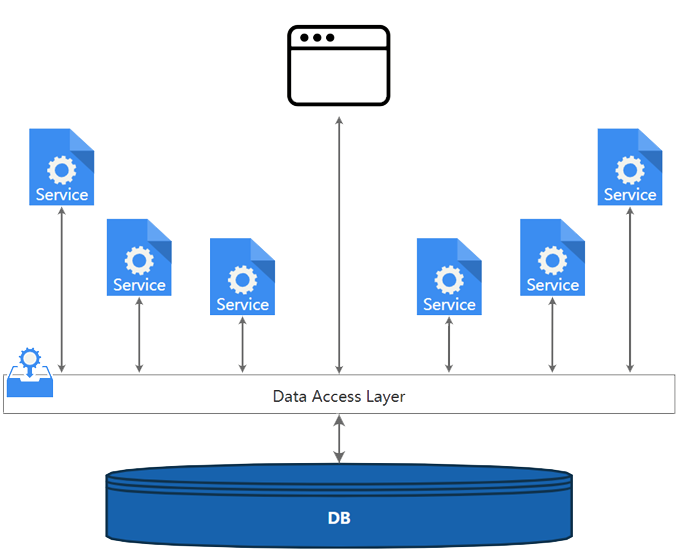
\includegraphics[scale=0.8]{4.png}
		\caption{DOA的拓扑结构}
		\label{fig:fig4}
	\end{figure}

	面向对象的软件体系结构有如下两个特点:
	\begin{enumerate}
		\item[(1)] \textbf{组件始终是无状态的:}DOA不需要按照集中管理的全局模式来描述数据或状态层,而是对每个相关组件进行组合和联合数据存储;
		\item[(2)] \textbf{组件之间交互最小化:}数据全部被储存在同一个数据库。系统可以直接查询数据库来获取价格,而不是通过特定的API向特定服务(或一组服务)请求价格。
	\end{enumerate}
	
	\subsubsection{面向对象的软件体系结构(DOA)的优势}

	面向对象的软件体系结构有两点优势:
		\begin{enumerate}
		\item[(1)] \textbf{开销成本:}DOA的成本开销是线性的而SOA的开销成本是二阶的。DOA模式下若更改某个服务,最多可能需要更改$N$个组件,而SOA模式下若更改某个服务,最多可能需要更改$N^2$个组件。随着组件数量$N$的增长,集成复杂度也随之增长,当$N$很大时,DOA的成本开销要远远小于SOA;
		\item[(2)] \textbf{数据安全性:}SOA要求所有服务的环境均是一致的。由于SOA服务通常是可独立寻址的,因此环境一致性要求每个服务必须与环境中的每个其他服务达成一致。RPC,pubsub和数据流可能会从一种环境泄漏到另一种环境。
		在DOA中,环境的概念要简单得多。知道一个组件连接到哪个数据存储层就足以描述它所处的环境。由于所有组件内部都没有存储状态,因此按定义隔离了数据。由于组件仅通过数据存储进行通信,因此没有将数据从一个环境泄漏到另一个环境的危险。
	\end{enumerate}
	
	\section{面向数据的软件体系结构的研究成果与进展}
	
	\subsection{数据注册中心机制}
	数据注册中心(DRC)是DOA的核心部件,通过它来构建逻辑的数据资源池,并管理数据和提供数据服务。DRC按照统一标准进行设计,可以将各个行业或不同规模的DRC进行互联和关联,从而构成更大规模的DOA系统\cite{apriori}。
	\newline
	
	\noindent\textbf{(1) 数据注册内容定义及元数据标准}
	
	广义数据包括云中存储的各种类型的数据,也包括互联网中传递的实时变化的数据,还包括物理世界存在的实体对象和状态所表征的数据。数据注册的内容包括数据特征、数据名称、存在位置、数据描述、数据属性、数据权限等。需要制定统一的数据注册元数据标准。
	\newline
	
	\noindent\textbf{(2) 数据属性信息定义}
	
	数据具有属性,例如数据权人(数据主人)、数据的生命周期、数据权限、数据状态、数据性质、数据合法性、数据质量等。
	\newline
	
	\noindent\textbf{(3) 数据分类及分类标准}
	
	包括数据分类的标准、分类的方法、分类的类别和分类的应用等。
	\newline
	
	\noindent\textbf{(4) 数据注册方法}
	
	包括数据注册方法,分为手动注册、半自动注册和全自动注册。在数据注册的同时,建立数据索引。应用产生的数据应自动进行注册。
	\newline
	
	\noindent\textbf{(5) 元数据索引和检索方法}
	
	数据注册中心是为应用提供数据访问服务的,访问效率取决于索引和检索方法。要建立高效的元数据索引和检索机制,开发高效的索引和检索方法。
	\newline
	
	\noindent\textbf{(6) 广义数据模式识别}

	数据注册中心注册的内容可以是广义数据,例如物理世界的实体。要快速检索这些广义数据,需要采取新的识别技术,例如可以采用基于模糊理论的模式识别技术来建立索引等方法。
	\newline
	
	\noindent\textbf{(7) 数据注册中心分布式部署模式}

	数据注册中心的数据注册信息可以非常大,因此数据注册中心也要部署到云的分布式环境中。DRC数据自动注册,数据注册内容随需自适应,并对历史数据进行注册与管理,鉴定数据来源及保障数据唯一性。 
	
	\subsection{数据权限中心机制}
	数据权限中心(DAC)是DOA的关键部件,对数据的安全存储、传输及应用授权进行管理。对数据实行“天生加密,授权使用”的机制,将数据分成存储和传输时保持加密的“数据态”和在应用中授权使用时解密的“应用态”,充分保证数据的安全及使用的授权。DOA从架构角度通过DAC来保障数据的安全性。DAC通过数据权限的管理对数据进行保护,并提供数据授权使用的机制,也可以保护数据拥有者的利益。
	
	数据权限中心的研究内容包括:数据合法性鉴定,数据使用记录及溯源,数据计帐,多级授权及认证,单个数据与批量数据或大数据量授权使用,密钥体系,数据透明加解密策略和算法,加解密效率与安全性及授权过程的妥协关系,传统数据传输加密技术适应性,应用环境安全保障,数据非法使用识别及数字水印技术,数据权人权利和知识产权相关问题等。
	
	数据权限中心要与数据注册中心配合,有关数据的属性和权限等数据,需要在数据注册中心进行注册和登记,数据权限中心根据注册的信息,对数据进行监控、授权、回收权利、认证、计帐、加解密和新数据安全属性注册等操作\cite{la}。
	
	\subsection{G/S模式}
	G/S模式, 即通用浏览器/服务云模式,是一种DOA架构下的数据交换模式与服务体系结构。涵盖了DOA架构中的客户端和服务端及其数据信息交换模型。通用浏览器指的是各种用千数据采集或数据展示的终端,如台式电脑、手机、平板等;空间信息服务器主要是指DOA架构中的服务器端,负责对数据进行管理,为客户端提供服务。G/S模式通过“请求-服务-聚合”的工作机制,综合运用多终端协同、智能缓存与时空可视化等技术,充分发挥了当前各种终端设备的存储、计算和图形处理能力,建立基于XML的行业数据交换标准, 实现了各行业、各异构系统之间数据的共享与交互\cite{lb}。
	
	DOA架构下G/S模式是一种新颖的数据服务模式, 其优势在于为多终端提供统一数据规范与整体架构,实现服务的按需聚合,与传统的信息服务模式相比有如下特点:
	\begin{enumerate}
		\item[(1)] 	\textbf{开放统一的数据标准:}G/S与C/S、B/S的本质区别就是建立了统一数据规范,以X\\XML的方式对各行业数据进行标识, 极大促进数据共享,提高数据的使用价值;
		\item[(2)] \textbf{客户端聚合服务:}随着终端设备性能不断加强, 利用当今终端设备强大的图形图像处理和计算能力,分出一部分数据处理的任务在客户端处理,客户端向服务器请求数据并聚合服务,对各行业数据进行统一调度与传输,最终在客户端完成任务;
		\item[(3)] \textbf{面向各行各业:}由于G/S 模式采用了开放的标准, 所以针对各行业领域应用,都增强了通用性。空间信息服务涉各行各业,使得人人都可以获得像自来水一样方便的服务。
	\end{enumerate}
	
	\subsection{面向数据的碎片化应用系统构建方法}
	面向数据的应用构建方法是一种以数据为核心,以应用单元的组装为主线的软件开发模型。该方法颠覆了传统开发模式,不强调软件的生命周期,而是数据生态系统。数据是有生命的,同一数据可以支撑不同的应用,不同应用的堆积和相互联系构成数据生态系统。由此建立的系统是生态、变化、和可持续发展的,老系统的数据导入到新的数据资源池,并在新的数据资源池上开发小应用,不断积累小应用,缓慢和逐渐替代原有系统,强调应用系统应该是从无到有,从小到大,周而复始,层层堆积而来的,是“肥沃的数据土壤上生长着茂盛的应用森林”。 基于成长型数据生态系统的软件开发模式应该是边调研边开发,开发过程也就是系统的扩展过程,这种开发模式可以充分利用遗留资源,容易实现定制化开发,并通过数据整合已有系统。
	
	面向数据的应用构建方法与传统的软件开发方法相比,有如下特点:
	\begin{enumerate}
		\item[(1)]  \textbf{以数据流动为导向:}根据用户的需求,关注数据流向,封装业务逻据,标准化流程和交互接口,自底向上的构建。在需求分析阶段,按照领域需求将问题空间进行划分,体现自上而下分而治之的思想,在应用组装阶段,更似积木的堆积过程;
		\item[(2)]  \textbf{并行开发:}应用单元在一定程度上实现自治,具有很高的独立性,所以各模块的设计和开发人员都可以只关注自己熟悉或负责的领域,专注千自己的任务,提高开发效率;
		\item[(3)]  \textbf{迭代与持续开发:}迭代过程不仅适用千单个应用单元的开发,还适用于整个应用系统的创建,在各个迭代周期内,系统开发人员快速地设计、实现、测试单个应用单元,然后将以开发的应用单元按照系统需求组装成应用系统。在整个系统的开发周期内,数据应用单元的开发和集成持续进行,及时检测,快速调整;
		\item[(4)] \textbf{高度重用:}面向数据开发的整个过程都围绕着应用单元的管理、重构与组装进行,根据其自治性与独立性,只需做很小的适应性修改就可以复用,已从简单的代码重用上升到最大限度的软件复用。
	\end{enumerate}

	\subsection{分布式数据注册中心架构}
	随着DOA管理的数据资源池不断增大,导致数据注册中心(DRC)需要管理的元数据也急剧增加,现有的DRC存在着诸多瓶颈,诸如性能扩容瓶颈、功能扩展瓶颈、响应及时性瓶颈、均衡性瓶颈等,因此,提高DRC的可扩展性,对DRC进行扩容,保证分布式DRC的负载均衡性势在必行。
	
	DRC应当采用分布式部署,元数据管理使用分布式可扩展数据库,优先级元数据应当存储在分布式缓存中,并且分布式缓存应当实现负载均衡\cite{lc}。
	
	\begin{figure}[!htbp]
		\centering
		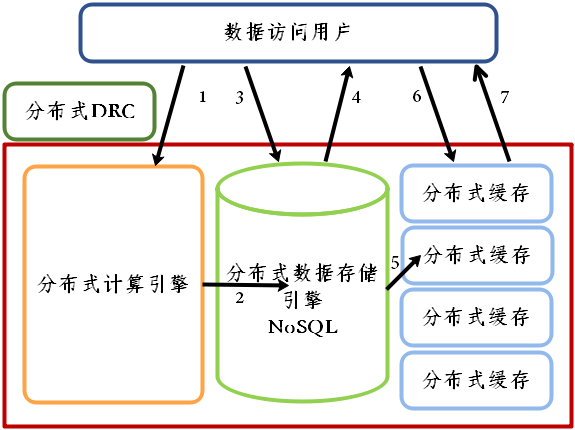
\includegraphics[scale=0.6]{5.png}
		\caption{分布式DRC架构模型}
		\label{fig:fig5}
	\end{figure}
	
	\noindent\textbf{(1) 分布式DRC伸缩性}
	
	所谓系统的伸缩性,就是指不需要改变系统的总体软硬件设计,仅仅通过改变部署的服务器数据量就可以扩大或者缩小系统的服务处理能力。只要做到了向系统集群中加入服务器的数量和集群的处理能力呈线性关系,那么系统就可以以此手段不断的提升自己的规模。传统数据注册中心采用单节点部署方式,硬件性能很难伸缩。
	\newline
	
	\noindent\textbf{(2) 分布式DRC扩展性}

	所谓系统的可扩展性,是指随着系统业务的增加和删减,系统在逻辑上能够灵活的进行功能的扩展和压缩。实际应用中,系统功能的增减往往需要更改数据库的字段,具体到DRC的功能扩展则常常需要对数据库中的元数据规范进行修改。传统的数据注册中心使用的是关系型数据库来存储元数据,字段的修改非常困难,分布式DRC架构模型中采用的是可分布式易扩展的非关系型数据库(Nosql) 数据库作为元数据的存储载体,极大地提高了DRC的扩展性。
	\newline
	
	\noindent\textbf{(3) 分布式DRC响应及时性}

	所谓系统的响应及时性,是指随着系统的存储数据的增加,在面对外部高并发访问时,系统依然拥有足够的响应带宽,能够高效及时的对外部请求做出响应。传统数据注册中心采用单节点部署,无论多么高级的服务器其响应带宽都是有限的,所以很难保证系统响应的及时性。分布式 DRC采用的分布式缓存架构 能够很好地提高DRC的响应及时性。
	\newline
	
	\noindent\textbf{(4) 分布式DRC的负载均衡性分析}

	所谓系统的负载均衡性,是指在集群系统在面对高并发访问和高任务处理时,集群中的各个服务器所承担的负载比是大致相同的。分布式DRC负载均衡的关键是保证分布式缓存的负载均衡。 
	
	\subsection{数据分区存储策略}

	分区是从数据时效上的可用性和资源区别分配上考虑的\cite{ld}。建立三段式的层次结构主要是考虑到两个方面的问题:
	\begin{enumerate}
		\item[(1)] \textbf{查询优化的考虑:}在大数据背景下,数据量庞大,纵然使用索引等技术查询也是很耗时的。针对时效大小分开,让更具有可能性的数据首先被搜索,这是在概率上避免在不必要的数据上消耗时间,从而达到查询上的速度优化和性能优化效果;
		\item[(2)] \textbf{资源开销:}在海量数据下,索引的维护开销是惊人的,首先是众多的索引会消耗大量的存储空间大,再者是过大索引会导致I/O操作频繁损耗性能。针对时效性分区的同时,也为时效性的判断开销的代价奠定了基础,系统中将资源的配置向高时效数据资源偏移。
	\end{enumerate}

	\subsubsection{数据三段式分区存储规则}
	数据处于三个区域的那个区域,根据时效值来划分,时效值代表的是数据在阶段时间上使用的情况,借此反应后续时间的数据使用趋势。具体规则如下面针对三个区域的三点:
	
	第一区是新入数据区,为防止插入数据的代价过高,这一区域大小固定。保存新注册进来的信息数据,新进来的数据无法判断时效性,考虑到统计数据中数据整体上有随时间质量下降的趋势,将其放在第一区域。这个区域是数据注册的接口,数据庞大数据插入开销过大。所以将可判定为高效的数据适时转出到高效或低时效数据区,对于数据注册的信息插入性能很有意义。
	
	第二区是高时效区域,大小不受限制。则是存储时效性上判定为第高时效的,在此区域的资源消耗系统紧缺资源消耗比较大。
	
	第三区域是低时效区域,这一数据区大小不受限制。属于冷宫区域,是数据陈放区域。
	\subsubsection{数据在个区域的转移规则}
	对于第一个新入数据区,有定时的转出,在数据量上相对平稳,不会存在数据积聚的情况。这一区域的根据查询在keywords上建立索引、在subject上建立索引。这一区域的数据来源是有注册方式。转出则包含两个方向,一个是第二层高效数据区,一个是第三层低效数据区。转出的方向依赖于存储管理模块根据时效算法的一个判定计算结果,T周期若时效性表现好,则进入高时效区域,否则进入低时效区域。
	
	对于第二区高效数据区域,这一区域数据也是有进有出,体积量也相对稳定。最坏的情况是所有数据的经常被使用,导致数据在此积聚。
	\subsubsection{三个区域的配置策略情况}
	针对三个区域的数据特点进行数据资源的分配,索引对于数I/O性能消耗,所以在配置上有所倾向。
	
	\section{DOA目前遇到的问题、展望}
	\subsection{DOA目前遇到的关键科学问题}
	
	\subsubsection{大数据时代下计算机软件体系结构的问题}
	大数据时代,计算机软件体系结构急需进行革命性的变革,以应对信息技术领域长期存在且在大数据时代愈发突出的问题,涉及到:信息共享,系统功能扩展,大数据管理,大数据分析和挖掘支持,软件工程,信息安全,数据企业利益保障等方面\cite{za}。虽然针对这些问题有着各种各样的解决方法和技术,但都不能彻底地或从根本上解决。现有的软件方法和软件体系结构,例如面向对象的编程( OOP,Object-Oriented Programming)解决的是复杂系统的编程方法问题,面向服务的体系结构( SOA, Service-Oriented Architecture)解决的是异构系统的服务调用和整合问题,基于构件的软件开发方法或面向构件的体系结构( COA, Component-Oriented Architecture)解决的是软件按组件方式的快速构建机制问题,它们都无法解决前述问题。
	
	\subsubsection{面向数据的软件体系结构对建立可持续发展的软件系统的支持问题}
	随着互联网技术的发展,大数据时代已经到来,数据资源成为一种商业资本,系统间的信息共享变得尤为重要。受当前软件体系结构的限制,软件开发长期存在的问题在大数据时代愈发凸显\cite{zb}。作为一个大数据时代下的软件体系结构,基于它所构建的大数据系统——我们定义为数据生态系统,应具有伴随数据的可持续发展的能力。推而广之,以面向数据,以数据为核心的软件体系结构(理论)来构建的软件系统及其计算机系统、信息系统的实现形式,也应该具有面向数据的可持续发展的能力。这也是我们需要探索和解决的科学问题。
	\subsubsection{面向数据的软件体系结构对数据保护与授权应用的支持问题}
	DOA通过数据注册中心,数据权限中心以及数据异常控制中心来统一定义、管理着这些由真实世界映射成虚拟世界的各种类型数据并提供相应的数据服务。其中数据权限中心是整个系统安全运行的保障,所有用户只有经过身份的认证和授权才能获取相应的数据服务\cite{zc}\cite{zd}。面向数据,就要以数据为核心,对数据进行保护,也要对应用进行支持。这种新的软件体系结构,为数据的安全、信息的安全、数据的应用、信息的应用等,带来了新的挑战和解决问题的新方法、新机制,这些都需要探索和解决。
	
	\subsubsection{面向数据的软件体系结构对应用增长和需求变化的支持问题}
	应用的不断增长和需求的不断变化,在面向数据的软件体系结构下应能够自动适应。这是新的机制、新的方法,需要深入研究和实现。
	
	\subsection{对DOA的未来展望}
	通过对面向数据的体系结构( DOA)进行理论和机制探讨, 为建立新一代的数据生态系统并从数据保护到数据的授权使用提供理论和方法技术支持。针对前述的信息技术领域长期存且在大数据时代愈发突出的七个方面的问题\cite{za}, 可以得到有效地解决:
	
	\subsubsection{信息共享}
	DOA 建立了以 DRC 为核心和以 DAC 为重点的数据资源池或数据大平台,所有的应用都“生长”在其上, 各应用系统都在一个“池子”里依照权限去获取所需的数据,各应用系统不需要去和其他应用系统去共享数据和信息, 因此没有信息“孤岛”和信息“烟囱”\cite{ze}\cite{zf},从根本上解决了信息共享的问题。如果两个以上的不同数据生态系统需要进行数据“共享”,只需将这些系统的 DRC进行相互认证和相互关联,不同的应用就可以在不同的数据资源池中找到所需要的数据了。
	
	\subsubsection{系统扩展}
	DOA 支持碎片化应用,因此,系统功能的扩展过程就是数据(应用)生态系统不断建设和发展的过程,数据可以不断积累,应用也可以不断增加和扩展。对于已有系统, 可以通过数据来进行整合。 将这些系统产生的数据不断“导入”到新的数据资源池中,再通过在数据资源池上不断开发和积累一些小的碎片化应用, 缓慢和逐渐替代原有系统, 完成从原来的应用系统到数据生态系统的过渡和迁移。
	
	\subsubsection{数据管理}
	DOA 是通过 DRC 以元数据方式,管理各种类型甚至包括网络空间和物理空间实时动态变化的数据,通过建立不同的分类方式和不同的数据索引检索方式,实现对数据的统一管理和提供应用服务支持。 通过 DRC、DEC 建立逻辑的数据资源池来管理数据并为应用提供服务,解决了数据唯一性保证和数据的一致性问题, 可以实现一个数据支持多种应用,丰富应用方式,避免数据冲突带来的严重后果。 这一点,在众多行业应用中都具有重要的意义,特别是在互联网和移动互联网的碎片化互动应用中, 更具有重要意义。 DRC本身也是利用云存储在分布式网络中,以应对大规模数据和大用户量及高并发访问,以保证数据访问的可靠性和高效性\cite{DeanMapReduce}\cite{gamesfromwithin.com}。
	
	\subsubsection{大数据分析和挖掘支持}
	大数据分析和挖掘需要有方便数据管理的架构,需要有方便和高效积累的数据\cite{Hey2009The}。 DOA 提供不断积累的、包含有中间计算结果的数据源泉,并提供成长型的数据生态系统和可行的数据安全管理机制, DRC提供快速和便捷的数据检索机制,并支持对复杂数据实现关联分析的算法, 可以基于 DOA 建立用于数据密集型大数据分析和挖掘的决策支持平台, 使基于大数据的预测、判断和决策更科学、客观和可持续\cite{KirkpatrickBig}。
	
	\subsubsection{软件工程}
	DOA 以数据为核心, 建立的数据资源池可以适应任何数据变化,也可以应对任何业务需求的变化。在 DOA 支持下,传统的面向业务的软件工程将转变为面向数据的软件工程\cite{tuzipei.baijia.baidu.com}。它迎合、满足、解决未来对于大数据及其应用分析挖掘不确定性的平台需求。在种种不确定下,仍然能够让用户自己就能快速简单地管理与分析不断变化与增长的数据,完成传统应用软件、传统中间件做不了的事情。它颠覆传统,不强调软件生命周期,而是强调数据生态系统,即数据大平台与碎片化应用系统,建立的是“肥沃的数据土壤上生长着茂盛的应用森林”;不考虑数据共享问题;是将业务逻辑转化为数据逻辑的开发过程;是基于成长型数据生态系统的应用软件开发模式;数据资源池的框架建立好后, 边调研边开发,开发过程就是系统扩展过程;是分阶段分期开发模式,可以保护已有投资,容易实现定制化开发。
	
	\subsubsection{信息安全}
	因为 DOA 建立的是数据“天生加密,授权使用”机制,这样可以使数据在开放环境下进行存储和传输,既可以适应传统封闭的安全环境下的应用,增强了信息的安全保障,又可以在开放环境下保证数据的安全和不被越权访问。传统的信息安全多是封闭环境下的信息安全,强调的是网络安全、系统安全和应用安全\cite{Labrinidis2012Challenges}。DOA 安全理念和技术,与现在发展的网络空间安全、系统安全、应用环境安全等技术相结合,可以有效提高信息安全保障。
	
	\subsubsection{数据提供者利益保障}
	数据必须经过授权才能够使用。 DOA 数据的使用过程就是数据的授权过程。通过计帐机制和计费手段,以及数据授权使用溯源机制,可以充分保障数据提供者的利益,也使得互联网和大数据时代的信息交易、数据应用等变得有序和有法可依。
	

	\section{总结}
	经过以上的分析和介绍,并结合苗放在论文\cite{apriori}中的观点,得出以下结论:
	\begin{enumerate}
		\item[(1)] DOA是数据思维和数据世界观的产物,在云计算的支撑下,从软件体系结构上解决问题,突破现有软件体系结构的局限性,为大数据的研究、发展和应用奠定了重要的基础;
		\item[(2)] DOA采用“面向数据和以数据为核心”的思想,通过DRC、DAC、DEC实现数据的统一定义和管
		理,通过DAUs 实现各种应用的管理和服务,建立数据大平台与碎片化应用的数据生态系统;通过数据
		“天生加密,授权使用”,建立从数据保护到授权应用的整套机制;
		\item[(3)] 基于DOA的示范项目初步应用表明,面向数据的体系结构能有效解决大数据时代面临的信息共享、系统功能扩展、数据管理、大数据分析和挖掘支持、软件工程、信息安全等软件体系结构方面的问题和挑战;
		\item[(5)] 随着大数据时代的来临,以往的传统的软件体系结构很难适应大数据场景下的需求,容易视系统具有不良的设计特征,同时给系统功能性需求的改变带来难度和较高的成本,这意味我们应该积极探索适应大数据应用场景的软件结构体系,这方面的研究国内仍有很大空白。
	\end{enumerate}
	
	
	\bibliography{reference/ref.bib}

\end{document}